\documentclass{article}
\usepackage[utf8]{inputenc}
\usepackage{graphicx}
\usepackage{hyperref}
\usepackage{listings}
\usepackage{float}
\usepackage[T2A,T1]{fontenc}
\usepackage[russian,french]{babel}
\usepackage{tikz}
\usepackage{amsmath}

\begin{document}
\title{Données Séquentielles et Symboliques: Translittération automatique}

\author{Alexandre Bérard, Mathias Millet, Charles Robin}
\maketitle
\begin{abstract}
\end{abstract}
\vspace{0.5em}
\section{Introduction}

La translittération est le fait de remplacer chaque graphème d'un système d'écriture par graphème ou un groupe de graphèmes d'un autre système, indépendamment de la prononciation. La translittération peut être par exemple utilisée pour écrire un nom propre d'un alphabet dans un autre. 

La translittération automatique est un domaine particulier de la translittération, qui va trouver des application par exemple pour traduire des mots qui ne sont pas encore dans les dictionnaires, ou traduire automatiquement des requêtes effectuées dans des systèmes d'écriture peu utilisés sur internet \cite{Singh2010}.


\subsection{Jeux de données}
Les données nous ont été fournies par Vincent Claveau. Nous disposons de deux jeux de données, concernant respectivement la translittération de l'\emph{espagnol} au \emph{portugais} et de l'\emph{anglais} vers le \emph{russe}. Chacun de ces jeux de données est divisé en deux fichiers, un fichier pour l'apprentissage et un fichier pour l'évaluation. Le fichier d'apprentissage contient plusieurs milliers d'entrées (3057 pour le portugais, et 7262 pour le russe), chaque entrée correspondant à un mot dans la langue originale et sa transcription dans le langage cible. Les entrées dans le fichier d'évaluation, elles, peuvent cependant contenir plusieurs transcriptions pour un même mot. 


\begin{figure}[H]
\caption{Entrées dans le fichier d'apprentissage Espagnol-Portugais}
\begin{verbatim}
2996: #fotocopiado# #fotocópia#
2997: #hexanoles# #hexanóis#
2998: #catalasa# #catalase#
\end{verbatim}

\caption{Entrées dans le fichier d'évaluation Espagnol-Portugais}
\begin{verbatim}
182: #centrifugación# #centrifugação#	other	unknown
183: #centriolo# #centríolo# OR #centríolos#	other	unknown
184: #ceramida# #ceramida# OR #ceramidas#	other	unknown
\end{verbatim}
\end{figure}


\begin{table}[H]
\caption{Longueur moyenne des mots dans chaque langue}
\begin{center}
\begin{tabular}{|l|c|c|}
\hline
Langue&Longueur moyenne\\
\hline
Espagnol&11.74\\
\hline
Portugais&11.52\\
\hline
\hline
Anglais&12.27\\
\hline
Russe&11.64\\
\hline
\end{tabular}
\end{center}

\end{table}


\subsection{Processus d'évaluation}
\label{eval}
\paragraph{Ensembles de test et d'apprentissage}
Comme nous disposons de données de test et d'apprentissage, la question de la méthode d'échantillonage à utiliser ne se pose pas.

\paragraph{Métriques d'évaluation}
Nous devons choisir une métrique afin de mesurer les performances de nos classifieurs, et fournir une moyen de comparaison (avec d'autres classifieurs, une baseline, ou un opérateur humain).
Nous mesurons la précision de notre système, c'est à dire la proportion de mots correctement traduits. Cependant, ce n'est pas suffisant car si la transcription choisie n'est pas correcte, il se peut qu'elle ne soit pas loin de la vérité.

Le même problème se pose dans la traduction automatique, de manière encore plus accentuée car le vocabulaire est beaucoup plus grand et les candidats de traduction sont souvent bien plus nombreux. Même dans les systèmes de traduction modernes, il est très fréquent que la traduction comporte au moins une erreur sans toutefois empêcher la compréhension de la phrase traduite. Une métrique couramment utilisée dans ce type de système, est le \emph{Word Error Rate}, qui est une distance d'édition (Levenshtein) adaptée aux phrases\footnote{On compte le nombre de mots qui diffèrent.}.
Aussi, pour notre système de translittération nous utiliserons une distance de \emph{Levenshtein}\footnote{Nombre minimal d'insertions, suppressions ou substitutions de lettres dans le mot original pour obtenir le mot cible.} pour évaluer la distance entre la proposition de notre système et la/les transcription(s) attendu(es).

Dans les données de test, les mots peuvent posséder plusieurs transcriptions acceptables. Dans ce cas, on mesure la distance au mot le plus similaire à la proposition du système.

$d(x,y) = \min_{y' \in traductions(x)} \{\delta(y,y')\}$

où $\delta(y,y')=levenshtein(y,y')$

Pour la précision, nous jugeons que la transcription est correcte si elle est égale à une des transcriptions possible.

Ces deux métriques donnent un résumé acceptable des performances du système.

\section{Règles de substitution}
Nous avons observé que dans le cas de l'espagnol et le portugais, les mots sont très similaires dans les deux langages. Dans les données d'apprentissage, la distance d'édition moyenne entre un mot espagnol et sa transcription en portugais est de \emph{2.0}.
Lorsque nous utilisons, comme \emph{baseline} pour notre système de translittération, un système qui se contente de renvoyer le mot original, nous obtenons donc une précision de \emph{51.0\%} et une distance d'édition moyenne de \emph{1.06} (au mot le plus similaire dans les candidats).

\paragraph{}
Nous avons ensuite constaté qu'un système mettant en jeu les trois règles de substitution suivantes (que nous avons sélectionné manuellement), obtenait une précision de \emph{58.6\%}, et une distance d'édition moyenne de \emph{0.76}.
\begin{verbatim}
is#->e#
ción#->ção#
ido#->ídeo#
\end{verbatim}
La progression est flagrante, avec seulement trois règles. Cela nous a amené à penser qu'un système sélectionnant automatiquement des règles de substitution basiques, pourrait obtenir de très bons résultats.

\subsection{Application des règles}
Dans le fichier de règles, les règles sont listées par ordre de priorité. Lorsqu'un mot doit être traduit, on tente d'abord d'appliquer la première règle, puis la deuxième, etc.  L'application d'une règle est simplement la substitution dans le mot de toutes les occurences de la partie gauche de la règle par la partie droite de la règle. Afin d'éviter les incohérences, nous prenons soin de ne pas appliquer une règle sur une portion du mot qui a déjà été modifiée. Si la règle chevauche une partie modifiée par une autre règle déjà appliquée, elle est tout simplement ignorée.

\subsection{Apprentissage}
\paragraph{Alignement}
Pour l'apprentissage de règles, nous commençons par aligner toutes les données d'apprentissage. Comme les mots sont très similaires, nous utilisons une simple distance de Levenshtein: l'alignement est construit à partir de la séquence d'opérations qui minimise la distance d'édition\footnote{Il y a quatre types d'opérations: \emph{égal}, \emph{insertion}, \emph{suppression}, \emph{substitution}. Les lettres successives concernées par des opérations \emph{égal} sont regroupées. Et les trois autres types d'opérations sont regroupés. Dans l'exemple, la lettre 'i' subit une \emph{suppression}, et la lettre 's' une \emph{substitution} par 'e'. Dans le résultat, 'is' est aligné avec 'e'}.
Un alignement se présente sous la forme suivante:
\begin{verbatim}
[('#catars', '#catars'), ('is', 'e'), ('#', '#')]
\end{verbatim}

De cet alignement, on pourrait déduire la règle simple: \verb|is -> e|. Seulement, cette règle est beaucoup trop générale, et possède probablement un taux de confiance faible. Il est possible cependant que les règles \verb|sis -> se|, ou \verb|is# -> e#| soient plus fiables.

D'un autre côté, si la règle \verb|catarsis -> catarse| est très fiable, son utilité est très discutable. En effet, elle revient a faire de l'apprentissage par c\oe{}ur, et n'a aucun pouvoir de généralisation.

L'objectif est donc de produire des règles ayant un bon compromis entre \emph{fiabilité} (qui sera évaluée par un \emph{taux de confiance}), et généralisation (évaluée par la longueur de la règle, et son \emph{support}).

\paragraph{Génération des candidats}
La production des règles se fait donc en énumérant, pour chaque alignement dans le corpus d'apprentissage, la liste des candidats de partie gauche de règle. Dans le cas de l'exemple, la liste des candidats est: \verb|['is', 'sis', 'is#', 'sis#', ...]|. Seuls les candidats de longueur supérieure au seuil $l$ sont conservés. Les candidats sont générés à partir des parties du mot dont l'alignement diffère, en étendant itérativement vers la droite et vers la gauche.

\paragraph{Calcul du support}
On calcule ensuite le support de chacun de ces candidats sur l'ensemble des données (\verb|len([w for w in words if 'is' in w])|).
Les candidats avec un support supérieur au seuil $s$ sont conservés. Cette étape permet de s'assurer que les règles sont suffisamment générales, et aussi de réduire le temps d'exécution (car l'étape suivante est beaucoup plus coûteuse).

\paragraph{Taux de confiance}
L'étape suivante est la génération de partie droite de règle. En parcourant l'ensemble de données, on calcule pour chaque candidat la partie droite de règle offrant le meilleur taux de confiance. Si ce taux de confiance est au-dessus du seuil $c$, alors la règle est conservée.

Par exemple, la règle \verb|is -> e| est jugée incorrecte pour l'alignement suivant: \verb|[('#hist', '#hist'), ('o', 'ó'), ('ria#', 'ria#')]|. En effet, le motif \verb|'is'| y est traduit par \verb|'is'|, et non \verb|'e'|.
De la même manière, pour l'alignement suivant: \verb|[('#imagina', '#imagina'), ('ción', 'ção'), ('#', '#')]|, la règle \verb|nac -> naç| est incorrecte, car incomplète. Le taux de confiance d'une règle est calculé en divisant le nombre de fois où la règle est jugée correcte, par le nombre total d'occurences de la partie gauche de la règle.

\paragraph{Tri des règles}
La dernière étape est de trier les règles selon leur ordre de priorité. Les règles les plus spécifiques doivent être appliquées avant les règles générales (sinon elles ne pourront jamais être appliquées). Nous trions donc les règles par ordre de taille (décroissante), une règle ne pouvant pas être plus générale qu'une règle plus courte. En fonction de la valeur du paramètre $l$, cette approche peut donner \emph{+1\% à +2\%} en précision par rapport à un tri inversé.
Une piste d'amélioration pourrait être de considérer leur taux de confiance dans l'ordre de tri des règles.

\subsection{Résultats}
Le score maximal que nous parvenons à atteindre avec ce système est de \emph{69.0\%}. Ces résultats sont sur le jeu de données \emph{Espagnol-Portugais}.
\begin{table}[H]
\caption{Types de règles et résultats}
\begin{center}
\begin{tabular}{|l|c|c|}
\hline
Règles&Précision&Distance d'édition\\
\hline
Aucune&51.0\%&1.06\\
\hline
3 (manuel)&58.6\%&0.76\\
\hline
584 ($s=2, l=5, c=0.8$)&\textbf{69.0\%}&\textbf{0.58}\\
\hline
\end{tabular}
\end{center}

\caption{Valeur des différents paramètres et résultats}
\begin{center}
\begin{tabular}{|c|c|c||c|c|c|}
\hline
Support $s$&Longueur $l$&Confiance $c$&Précision&Distance&Règles\\
\hline
2&6&0.80&56.8\%&0.82&104\\
\hline
2&5&0.80&\textbf{69.0\%}&\textbf{0.58}&315\\
\hline
2&4&0.80&68.1\%&0.59&584\\
\hline
\hline
3&5&0.80&67.3\%&0.61&195\\
\hline
5&5&0.80&67.2\%&0.61&\textbf{128}\\
\hline
1&5&0.80&64.5\%&0.68&1490\\
\hline
\hline
2&5&0.75&68.5\%&0.59&340\\
\hline
2&5&0.85&68.4\%&0.59&287\\
\hline
\end{tabular}
\end{center}
\end{table}

Nous n'avons pas considéré l'utilisation de cette méthode sur les données \emph{Anglais-Russe}, car l'alphabet est complétement différent. L'hypothèse de similarité des mots dans les deux langages n'est donc plus vérifiée. D'autres méthodes sont plus adaptées, notamment les méthodes \emph{statistiques} (traduction statistique, CRF).


\section{Translittération statistique}
Le problème de la translittération est relativement proche de la traduction automatique. En traduction automatique, on traduit des séquences de mots d'un langage à un autre. Cela se caractérise par l'association à chaque mot (ou groupe de mots) de la phrase original, d'un mot (ou groupe de mots) dans le langage cible, avec un réordonnancement possible. En translittération, on associe des lettres ou groupes de lettres.

\begin{figure}[H]
\label{translation_alignment}
\caption{Traduction et translittération}
\centering
\vspace{0.3cm}
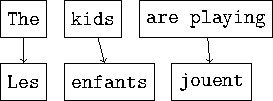
\includegraphics{word_alignment.pdf}
\hspace{0.5cm}
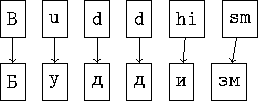
\includegraphics{letter_alignment.pdf}
\end{figure}

La différence essentielle, par rapport à la traduction automatique est l'absence de réarrangements dans le résultat. En effet, dans certaines paires de langages, les mots doivent être réordonnés (e.g. les adjectifs entre le français et l'anglais). Ce n'est pas le cas dans la translittération.

\paragraph{Traduction statistique}
L'approche de traduction automatique avec le plus de succès est la \emph{traduction statistique}. La traduction statistique se base sur la \emph{loi de Bayes}:
\begin{center}
$e = arg max_{e \in e*} p(e|f) = arg max_{e \in e*} p(f|e)p(e)$
\end{center}
Où $f$ est la phrase à traduire, $e*$ est l'ensemble des traductions possible, et $e$ la traduction choisie. La probabilité $p(e)$ est le \emph{modèle de langue}. Il s'agit de la probabilité d'observer la phrase $e$ dans la langue cible. $p(f|e)$ est le modèle de traduction et dépend de l'approche utilisée. Ces probabilités sont souvent estimées avec un \emph{maximum de vraissemblance} sur de larges corpus de textes alignés dans les deux langues.


La traduction syntagmatique (ou \emph{phrase-based traduction}), considère des \emph{syntagmes} comme unité de langage (\cite{Koehn03}). Un syntagme (ou \emph{phrase}) est un groupe de mots constituant une unité syntaxique (par ex., ``are playing'' est un syntagme). Les anciennes approches basées sur les mots se heurtaient à certaines difficultés, notamment pour traduire les expressions (par ex. ``kick the bucket''/``casser sa pipe'').

Dans le cas de la translittération, l'approche syntagmatique est également très intéressante. Dans la \emph{Figure \ref{translation_alignment}}, ``sm'' et son équivalent russe sont des syntagmes.

Dans notre travail, nous utiliserons donc le framework de traduction statistique (syntagmatique) \emph{Moses}, \cite{Koehn07}.

\subsection{Moses}
\paragraph{}
Nous devons dans un premier temps modifier les données, pour que Moses les considère comme des phrases. Pour cela il suffit d'insérer des espaces entre les lettres (chaque lettre est un mot). Pour empêcher tout réarrangement de mots (traduction monotone), nous mettons le paramètre \emph{distortion-limit} à la valeur $0$. Les résultats sont similaires, mais le temps d'exécution largement réduit.

\paragraph{}
Nous nous sommes inspirés du travail de \cite{Matthews}, où la translittération de noms propres (du corpus \emph{Gigaword}) est effectuée, en utilisant Moses.

\paragraph{}
La création d'un système de traduction avec Moses se fait en plusieurs étapes (manuel d'utilisation, \cite{Moses}):
\begin{itemize}
    \item Utilisation d'\emph{IRSTLM} (ou autre) pour générer le modèle de langue à partir des données de la langue cible (les mots du russe ou du portugais dans notre cas);
    \item Alignement des données avec \emph{Giza++};
    \item Création du modèle de traduction.
\end{itemize}

\paragraph{Paramètres}

Les paramètres d'apprentissage sont les suivants:
\begin{itemize}
    \item Ordre des N-grammes du modèle de langue (3 est la valeur retenue);
    \item Réordonnancement (monotone dans notre cas);
    \item Longueur maximale des phrases (par défaut 20, 5 donne d'aussi bon résultats);
\end{itemize}

Dans Moses, la probabilité finale d'une traduction est le produit de quatre probabilités: la probabilité du modèle de traduction syntagmatique, la probabilité du modèle de langue, le modèle de réordonnancement (qui n'est pas considéré dans notre cas), et finalement la pénalité de longueur. Les paramètres du modèle sont les poids attribués à ces différentes probabilités.

\subsection{Résultats}

\begin{table}[H]
\begin{center}
\caption{Valeurs optimales des poids}
\begin{tabular}{|l|c|c|c|}
\hline
Données&Pénalité de longueur&Modèle de langue&Modèle de traduction\\
\hline
ENG-RUS&-0.3&0.65&\verb|[1,0,1,0.2]|\\
\hline
SPA-POR&-0.7&0.35&\verb|[1,0,1,0.2]|\\
\hline
\hline
Par défaut&-1&0.5&\verb|[0.2,0.2,0.2,0.2]|\\
\hline
\end{tabular}
\end{center}
\end{table}

\begin{table}[H]
\caption{Résultats de la baseline (paramètres par défaut)}
\begin{center}
\begin{tabular}{|l|c|c|c|}
\hline
Données&Précision&Distance moyenne&Variance\\
\hline
ENG-RUS&59.1\%&2.10&15.41\\
\hline
SPA-POR&56.9\%&1.21&4.30\\
\hline
\end{tabular}
\end{center}

\caption{Résultats avec paramètres optimaux}
\begin{center}
\begin{tabular}{|l|c|c|c|}
\hline
Données&Précision&Distance moyenne&Variance\\
\hline
ENG-RUS&\textbf{67.8\%}&\textbf{1.75}&14.47\\
\hline
SPA-POR&\textbf{71.5\%}&\textbf{0.73}&3.46\\
\hline
\end{tabular}
\end{center}
\end{table}

\begin{figure}[H]
\begin{center}
    \caption{Histogramme des distances pour les données \emph{ENG-RUS}}
    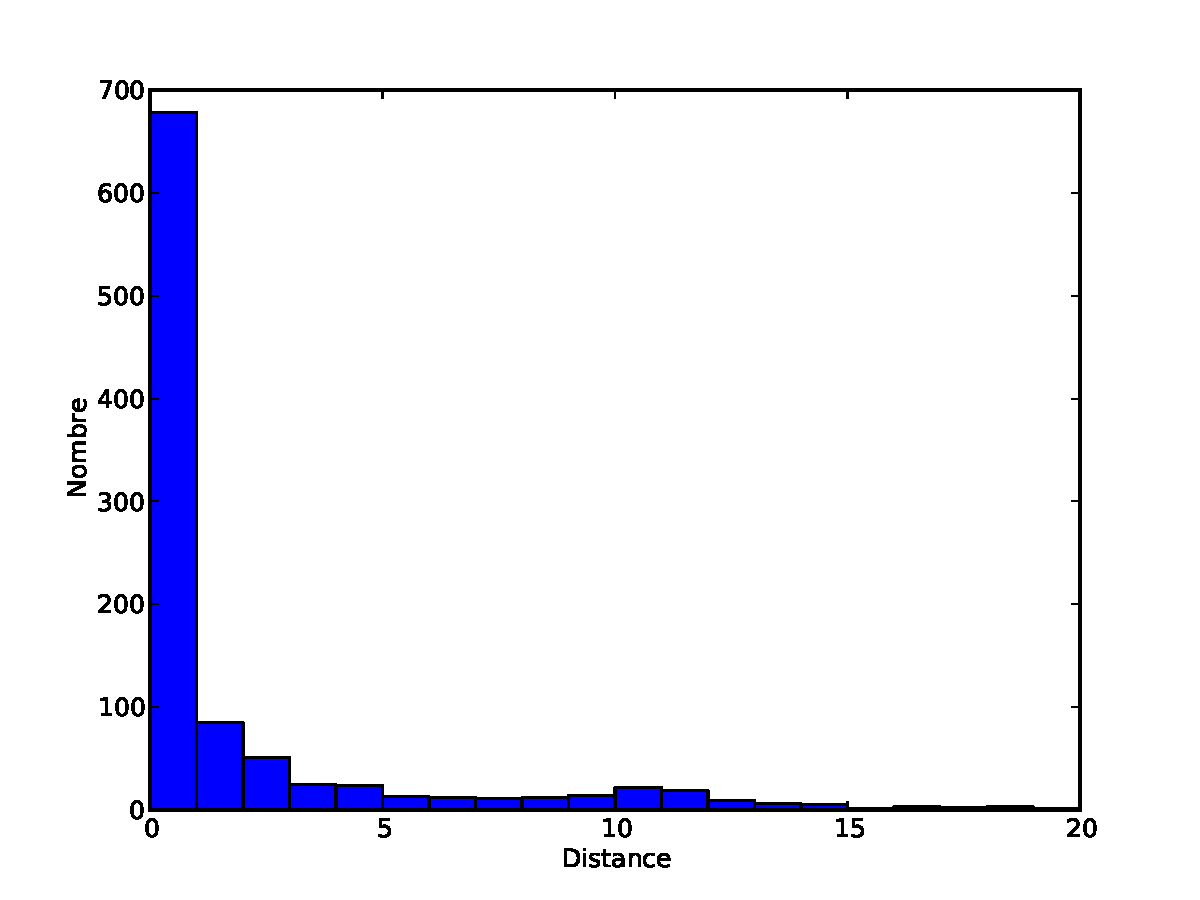
\includegraphics[scale=0.5]{moses_histogram_rus.pdf}
    
    \caption{Histogramme des distances pour les données \emph{SPA-POR}}
    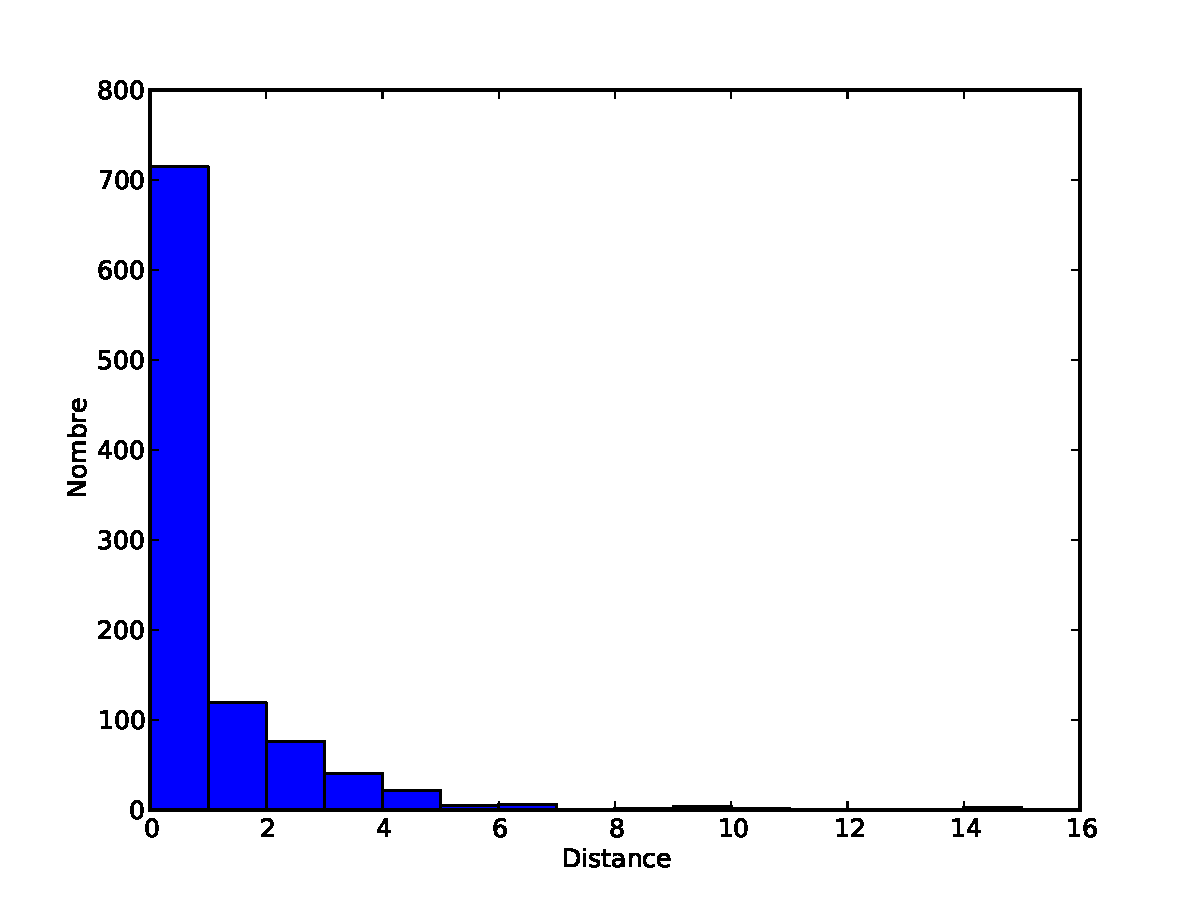
\includegraphics[scale=0.5]{moses_histogram_por.pdf}
\end{center}
\end{figure}

\section{CRF}
Les CRF \emph{Conditionnal Random Fields} sont des modèles statisitques permettant de prendre plus de contexte qu'un classifieur "ordinaire". Ils permettent l'étiquettage de séquences. Ils ont été introduit par \cite{Lafferty01}. L'équation principale des CRF est donnée à l'équation \ref{eqcrf}.
\begin{equation}
p(\textbf{s}|\textbf{o}) = \frac{1}{Z_0}exp(\sum_{t=1}^T\sum_k \lambda_k f_k(...))
\label{eqcrf}
\end{equation}
Les $f_k$ sont des fonctions \emph{feature} données par l'utilisateur nécessitant certains arguments, et les $\lambda_k$ sont des poids qui sont appris grâce aux données d'apprentissage, \textbf{s} et \textbf{o} étant respectivement une séquence d'état et la séquence des observations (ici les lettres). Les fonctions features sont des fonctions qui ont pour valeur 0 sur presque tout leur domaine et 1 sinon.

Nous avons utilisé dans le cadre de ce projet, l'implémentation CRF++\footnote{https://code.google.com/p/crfpp/}.

\subsection{Apprentissage}
Dans le cas de l'apprentissage des CRF, nous avons dû en premier lieu aligner lettre à lettre les mots et leurs traductions dans l'ensemble d'apprentissage. Pour celà nous avons utilisé l'algorithme \emph{dpalign} dont une implémentation en perl est disponible sur le site du cours. Nous avons ensuite donné ces données à CRF++ en plus d'un fichier \emph{template} décrivant les fonctions features que nous souhaitions utiliser. Nous avons choisi comme fonctions features des unigrammes. Le contenu du fichier template est le suivant :
\begin{verbatim}
# Unigram
U0:%x[0,0]
U1:%x[-1,0]
U2:%x[1,0]
U3:%x[-2,0]
U4:%x[2,0]
U5:%x[-3,0]
U6:%x[3,0]

# Bigram
B
\end{verbatim}

\subsection{Évaluation}
Nous testons ensuite le modèle CRF obtenu grace aux données de test, en suivant le protocole décrit à la section \ref{eval}. Il est important de noter qu'aucun alignement n'a été réalisé sur ces données, ce qui a pu poser quelques problèmes. En effet, il est possible d'étiquetter une et une seule étiquette par observation, il est donc impossible de traduire un mot par un mot plus long.

\subsection{Résultats}
Un récapitualatif de nos résultats est disponible ci-dessous sur le jeu de données \emph{Espagnol-Portugais}. Nous trouvons des résultats un peu moins bons que grace aux règles de substitutions, cependant ils sont meilleurs que notre baseline ainsi qu'avec les trois règles de substitutions trouvées manuellement.
\begin{center}
\begin{tabular}{|l|c|c|}
\hline
Règles&Précision&Distance d'édition\\
\hline
Baseline&51.0\%&1.06\\
\hline
3 subst.&58.6\%&0.76\\
\hline
CRF&\textbf{63.9\%}&\textbf{0.69}\\
\hline
\end{tabular}
\end{center}

\section{Conclusion et perspectives}
%\nocite{*}
\bibliographystyle{apalike}
\bibliography{report}

\end{document}
